We apply the estimation methods to proxies of two seperate systems: The Atlantic meridional overturning circulation (AMOC), where these methods were initially used \cite{Ditlevsen2023} and global climate variations.
\subsection{Estimating tipping of the Atlantic meridional overturning circulation with the $t$-diffusion based model.}
For the AMOC the time series we consider is the sea surface temperature (SST) anomaly in the subpolar gyre in the north Atlantic ocean in comparison to the the global mean SST anomaly. The SG SST minus twice GM SST has been argued to be a proxy of the strengh of the AMOC; we use twice the GM SST anomaly in compensation for the amplificaiton of global warming in the polar regions \cite[caption of figure 1]{Ditlevsen2023}.
\begin{figure}[h!]
    \begin{center}
    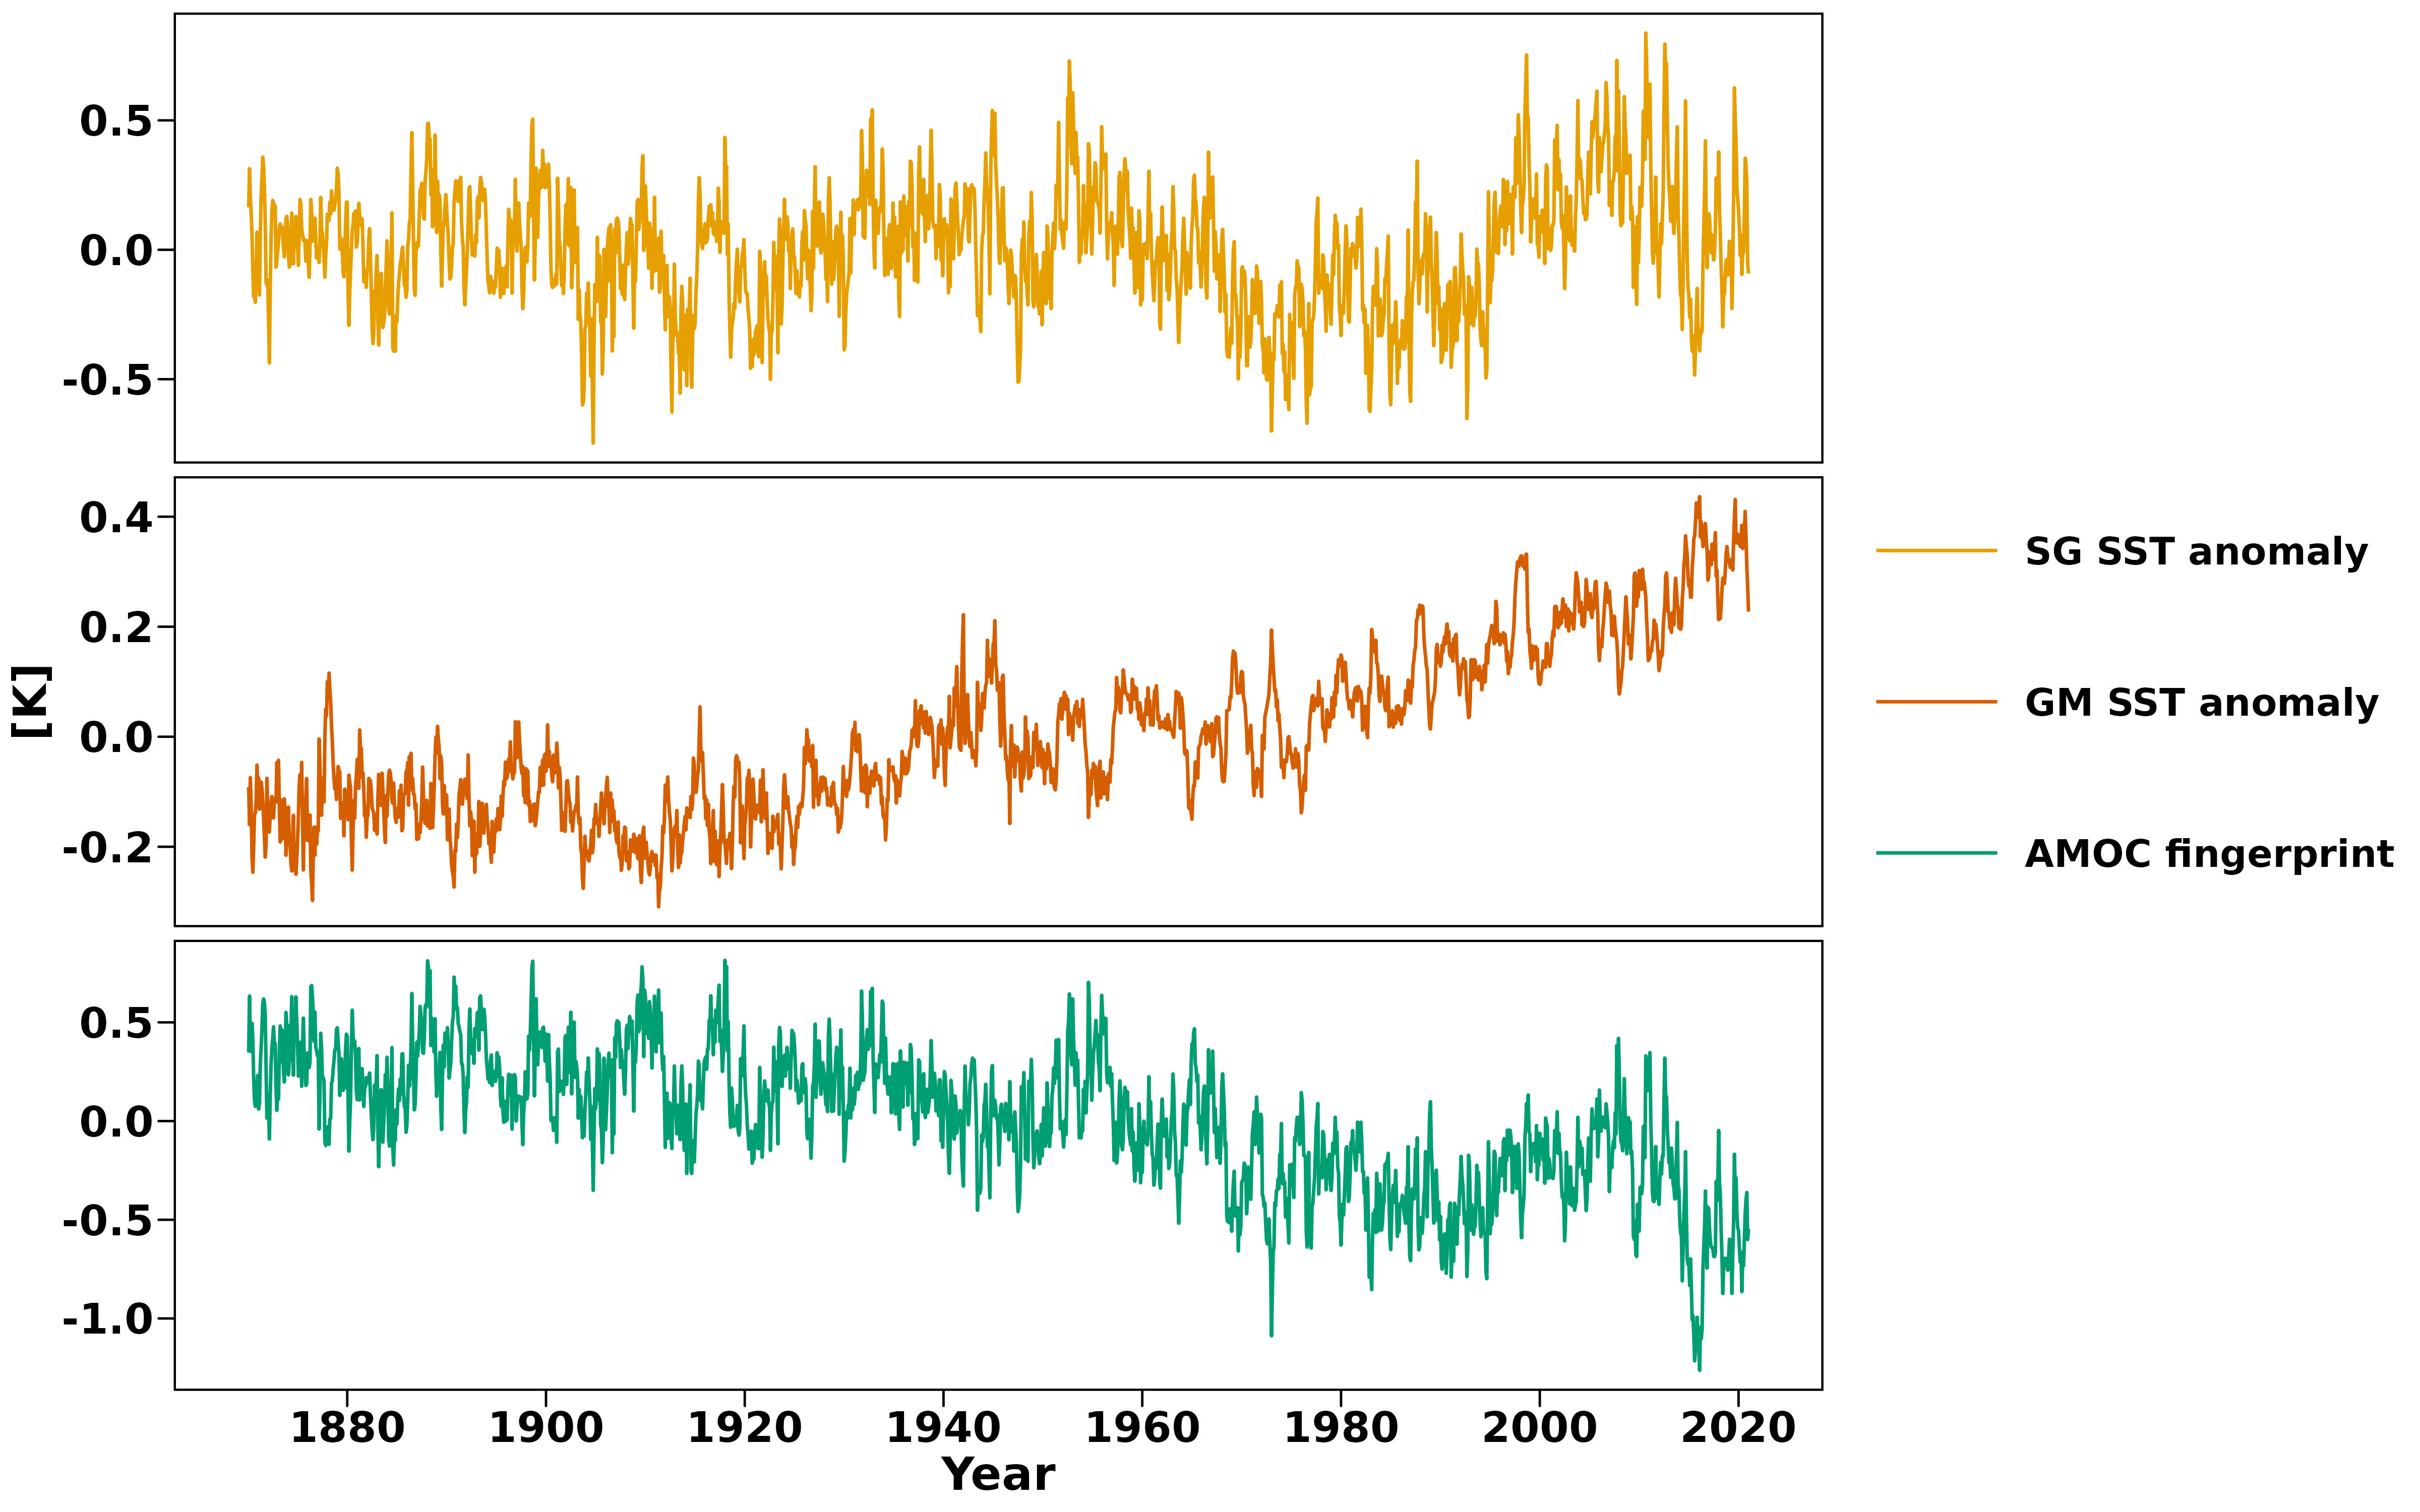
\includegraphics[scale = .075]{figures/AMOC_data_plot.jpeg}
    \caption{SST anomalies in the subpolar gyre and global mean as well as the AMOC fingerprint}
    \label{figure:AMOC_plot}
    \end{center}
\end{figure}\\
The fingerprint contains negative values, so without any transformations we can only employ the additive- or $t$-diffsion based models. Now, a version of the additive model with penalization has already been studied on the time series, thus we try to with the $t$-diffusion based model. Recall that relative to the additive model the $t$-diffusion based model has a stochastic term, which is alwaus greater than or equal. How this captures the AMOC-fingerprint remains to be seen though.
\subsubsection{Determining $t_0$ and estimating the tipping point}
We start by estimating parameters in the stationary- and dynamic parts of the process, before we can do that we must figure out, which part of the time series is in the respective parts. In the initial use of the methods it is determined to be $t_0 = 1924$. This is done by sweeping over values of a running window, and the start time of ramping, $t_0 \in [1910, 1950]$ used for a moment estimator of the tipping point; we do not consider this estimator in further detail, but instead propose an alternative method to arrive at $t_0$ that does not depend on an analysis of early warning signals. We sweep over the years $t_0 \in [1914, 1950]$ and estimate in the stationary - and dynamic parts. We then compare the normalized negative log-likelihoods. The minimum does not care about scaling of positive constants, but in order to be able to compare within models with diffferent sample sizes, we need to use the normalized negative log-likelihood. Because of their similarities for samples on a scale close to zero, we start each of the stationary parts of the processes in starting points corresponding to the approximate MLEs for the OU-process \cite[equation (S4-S6)]{DitlevsenSupplementary}. In the respective dynamic parts we initialize the optimization in $A = 1$ and $\tau = 2021 - t_0$ for each of the $t_0$'s. $A = 1$ is not necessarily the best starting value, but we have yet to come up with a good starting value for this parameter based on the data; albeit the choice is not completely arbitrary as it corresponds to a more parsimonious model. In addition, it is the value of choice in the original application \cite{Ditlevsen2023}. We choose $\tau$ in the above manner, because it is a lower bound for $\tau$. We have not observed tipping yet, thus $\tau$ is at least the difference between the largest year in the data: 2021 and the year when the initial ramping began. Sweeping over the years, we get a negative log likelihood as a function of $t_0$ for the respective parts.
\begin{figure}[h!]
    \begin{center}
    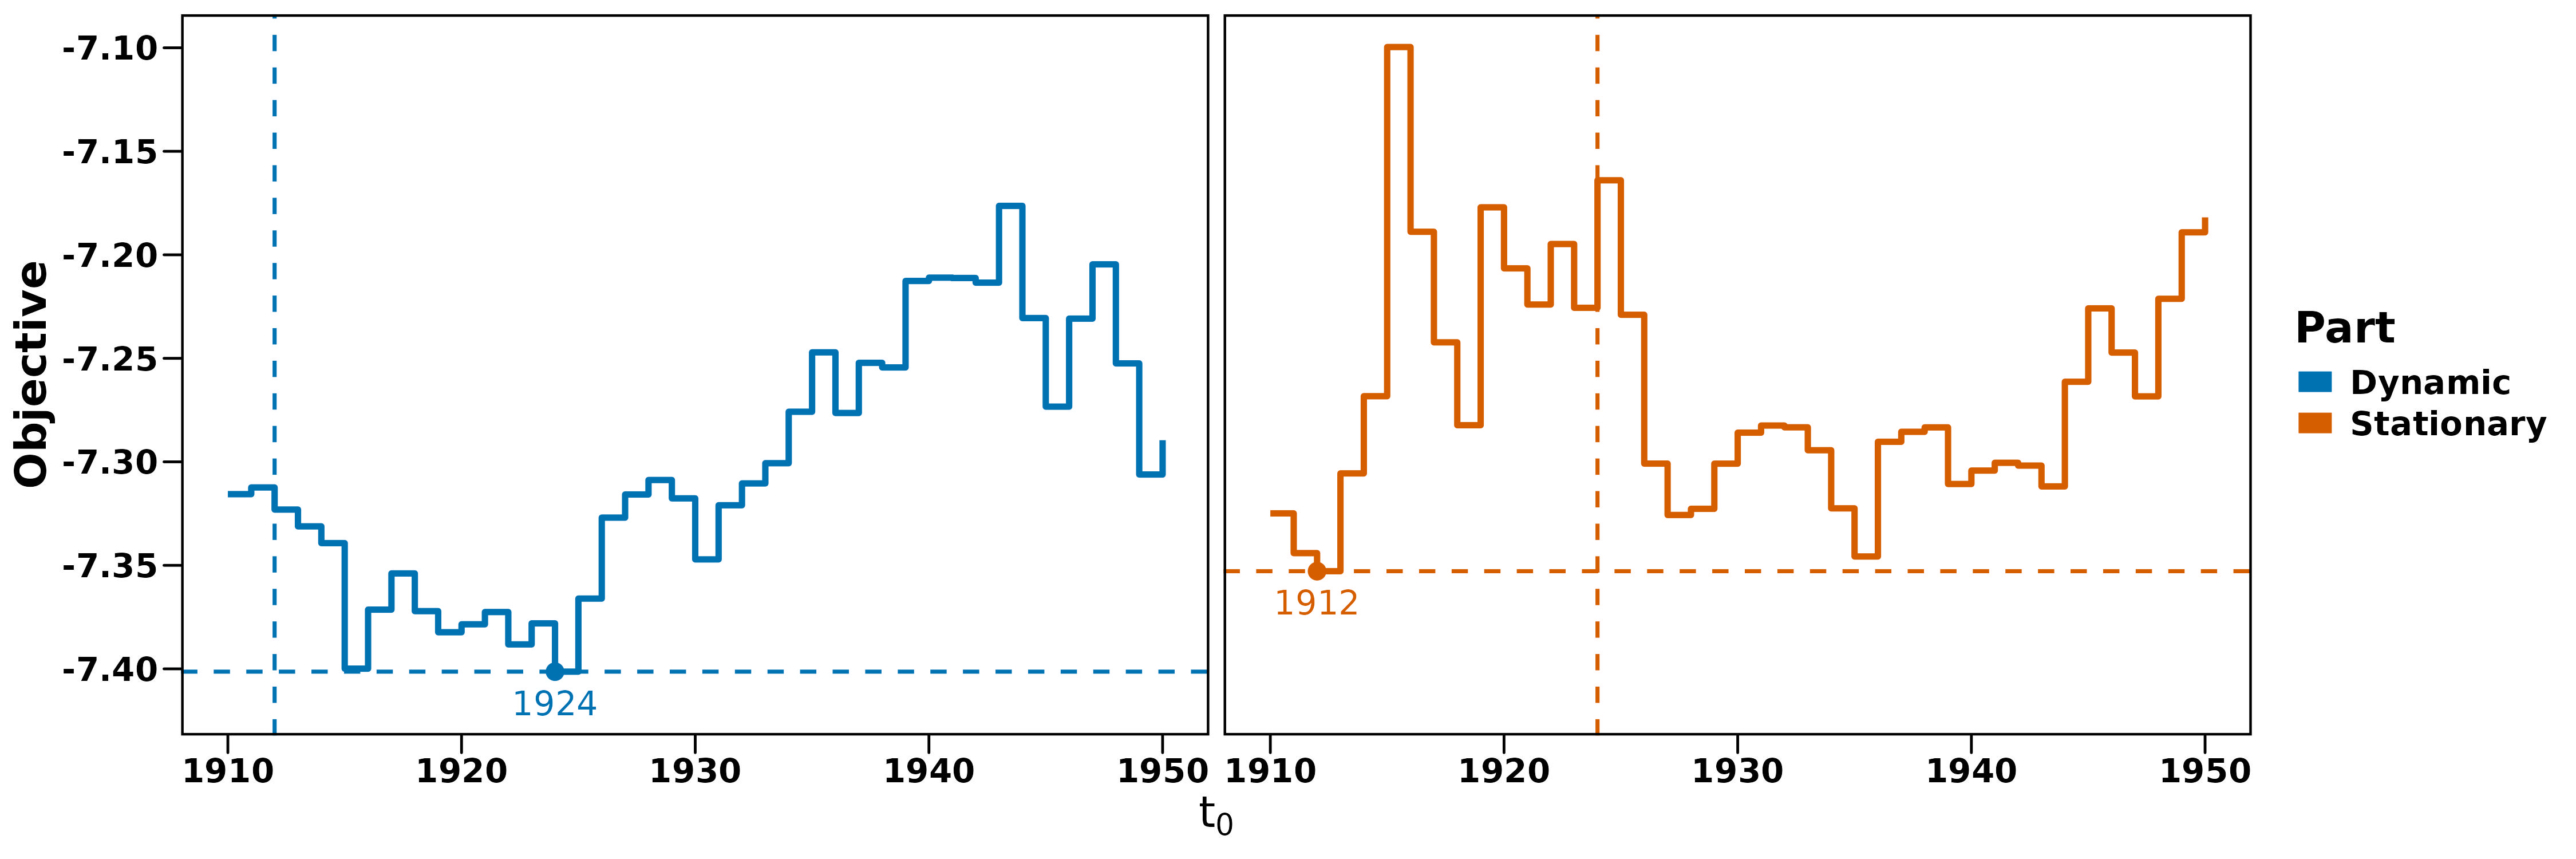
\includegraphics[scale = .095]{figures/ramping_year_likelihood_plot.jpeg}
    \caption{Negative log-likelihood for the stationary- and dynamic parts as a function of $t_0$.}
    \label{figure:negLoglikRamping}        
    \end{center}
\end{figure}\\
Where we have marked the minimal objective accross all $t_0$ for both the stationary- and dynamic parts. These are obviously not the same and to highlight this fact we have marked where the minimum is for one part onto the other by the vertical dotted lines. The horizontal lines are the values of the objective at the minimum $t_0$. Note that the $t_0$ that minimizes the objective for the dynamic part overall is the same as the one found in \cite{Ditlevsen2023}.\\
Still we would like to be able to decide independently between the two. One might be tempred to note that the objective values are rather similar scales numerically, but they are likelihoods for different types of models and thus not-comparable, meaning we cannot construct some sort of weighting between the two
When the minima are this far away from each other, the methods might seem to fall-short. Before we go into details about how we might remedy this, however, let us quickly consider what impact the two different $t_0$'s have on the estimated parameters. We take the estimated parameters from the sweep earlier and mark the two points in time where the stationary- and dynamic parts had their objectives minimizes overall
\begin{figure}[h!]
    \begin{center}
        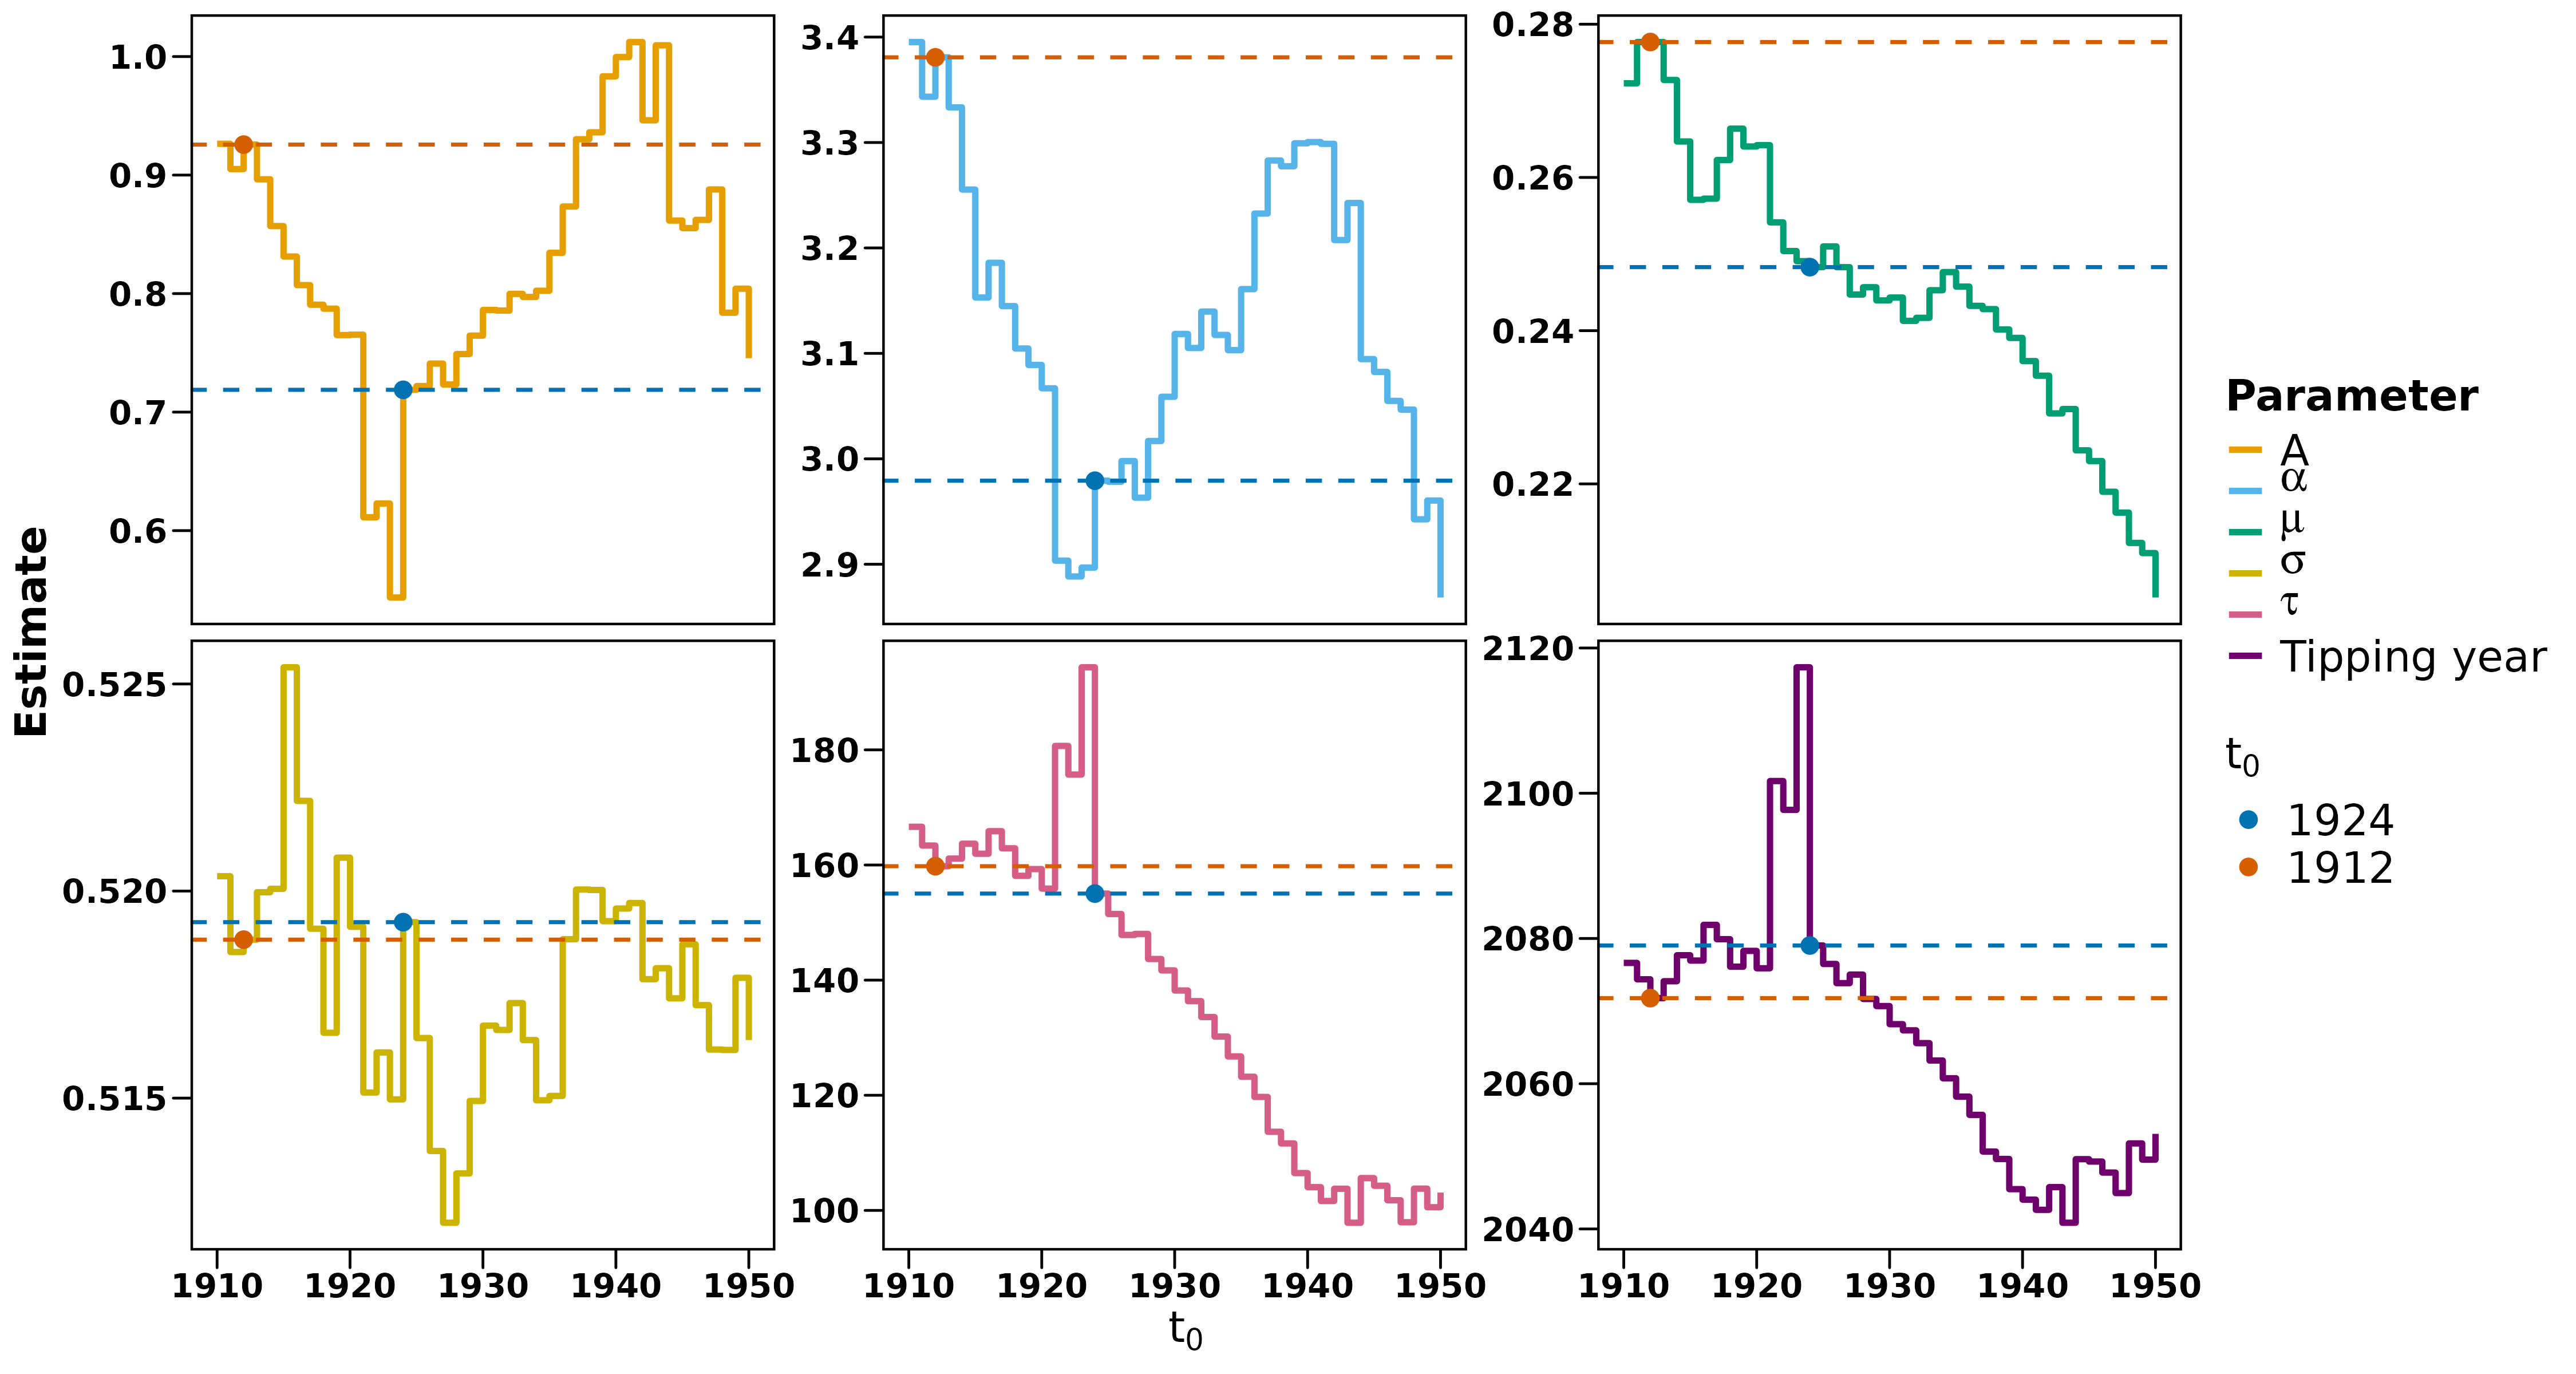
\includegraphics[scale = .09]{figures/estimators_full_plot.jpeg}
        \caption{Estimated values as a function of $t_0$ stratified after parameter - The points $t_0$ that overall minimized the dynamic- and stationary objectives have been marked by points.}
    \end{center}
    \label{figure:AMOC_estimates_t_0}
\end{figure}\\
Generally, the estimates from the two models seem to mosty align quite well. For this comparison the scale of the individual estimator of course matter so for a more clear direct comparison we tabularize the respective estimates at the two points and their relative differences
\begin{table}[h!]
    \centering
    \begin{tabular}{lllr}
     Parameter & Estimates 1924 & Estimate 1912 & Relative difference \\ \hline
    $\alpha_0$ & $2.98$ & 3$.38$ & $-11.88\%$ \\ 
      $\mu_0$ & $0.25$ & $0.28$ & $-10.58\%$ \\ 
      $\sigma$ & $0.52$ & $0.52$ & 0$.08\%$ \\ 
      $\tau_c$ & $155.03$ & $159.79$ & $-2.98\%$ \\ 
      Tipping year & $2079.03$ & $2071.79$ & $0.35\%$\\ 
      $A$ & $0.72$ & $0.93$ & $-22.35\%$ \\ 
       \hline
    \end{tabular}
    \caption{Parameter estimates from the stationary- and dynamic parts for the $t$-diffusion based model of the normal saddle-node form stratified after whether ramping time to minize the stationary- or dynamic negative log-likelihood is used.}
    \label{table:Estimates_t0_AMOC}
\end{table}\\
What was perhaps already clear is that the parameters $A, \alpha_0, \mu_0$ deviate a bit more from one another between the two $t_0$'s than the remaining parameters. To this end is very positive that the $\tau$-parameter, and addittionaly the tipping year have a very small relative difference; these are of course heavily correlated, but due to the different ramping start we do see the Tipping years becoming almost equal inspite of more different $\tau_c$, relatively speaking. This is naturally good news as it seems that the two model are almost in perfect agreement on the value of the parameter of interest. Still, we seek to find \textit{the} ramping time, and to do so we diagnose the two models. We calculate the uniform residuals for both the stationary- and dynamic part of the process for both $t_0$ and plot the QQ-plots for each part stratified after which $t_0$ was used.
\begin{figure}[h!]
    \begin{center}
        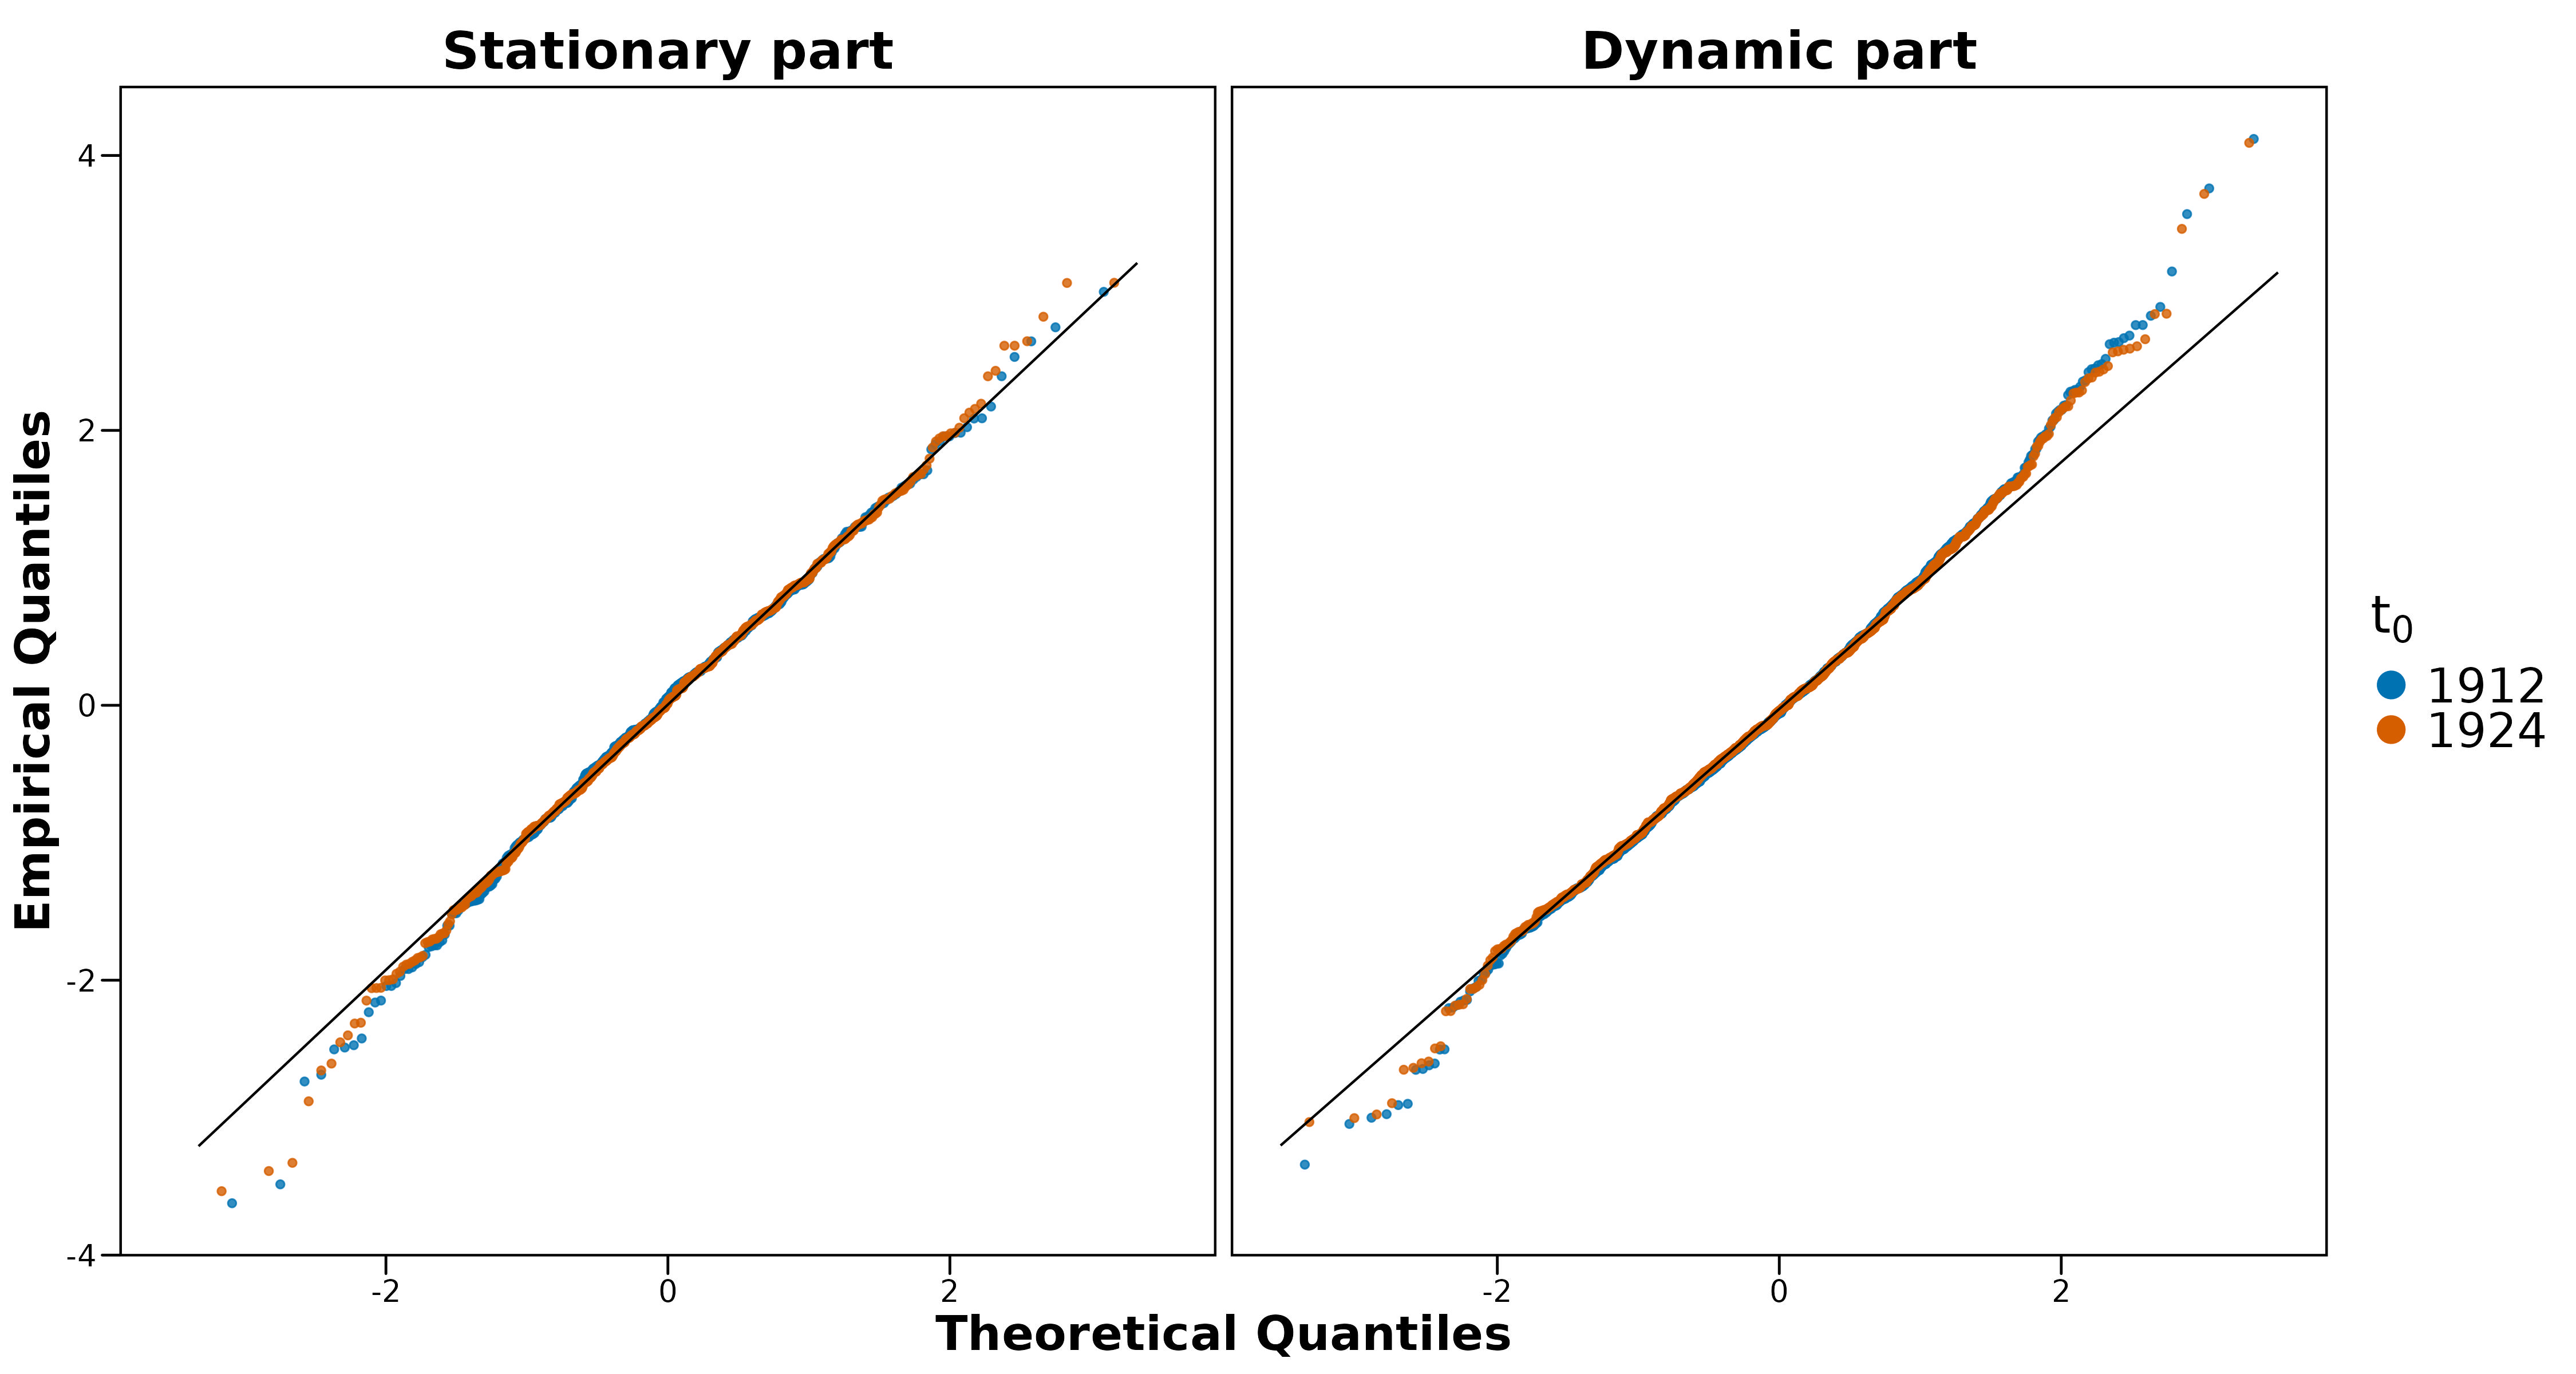
\includegraphics[scale = .09]{figures/QQ_plot_parts.jpeg}
        \caption{QQ-plots for the stationary- and dynamic parts grouped by the $t_0$ used.}
        \label{figure:AMOC_QQ_t_0}
    \end{center}
\end{figure}\\
Looking at the QQ-plot for the stationary part, we unsurprisingly see that the fit corresponding to $t_0 = 1912$ appear a bit better, ableit the two are hard to distinguish. Generally though, the empircal quantiles seem a bit heavy-tailed suggesting a slight lack of fit. Conversely, the fit in the dynamic part appear to be better when using $t_0 = 1924$. The difference between the two ramping values seems to be more pronounced here. Sometimes it can be a bit difficult to diagnose these fits due to a couple of extreme outliers. To illustrate this we tabularize the empirical quantiles and add the theoretical quantiles from the standard normal distributuon. In the core of the distributions there is not too big of a difference between the two $t_0$; though the overall impression is the same, so we move on with $t_0 = 1924$ and refer to table \ref{table:QQ_table_parts} in appendix \ref{section:benchmark} for the exact quantiles.
\subsubsection{Model evaluation and confidence intervals for the estimates}
Although we already have presented our diagnostics of choice for the model in advance qua the uniform residuals in figure \ref{figure:AMOC_QQ_t_0}, we have yet to assess the uncertainty of the parameters. Recall that our estimates correspond to the values in the \textit{"Estimates 1924"}-column in table \ref{table:Estimates_t0_AMOC}. We simulate using the $t$-diffusion based scheme in (\ref{eq:skew_t_sim}) with these parameters. Then we fit the model to the simulated data with the estimated parameters from the original data set as the starting values. Simulating $M = 2000$ realizations from the model and estimating in the respective parts, we get the following distribution of the estimates
\begin{figure}[h!]
    \begin{center}
    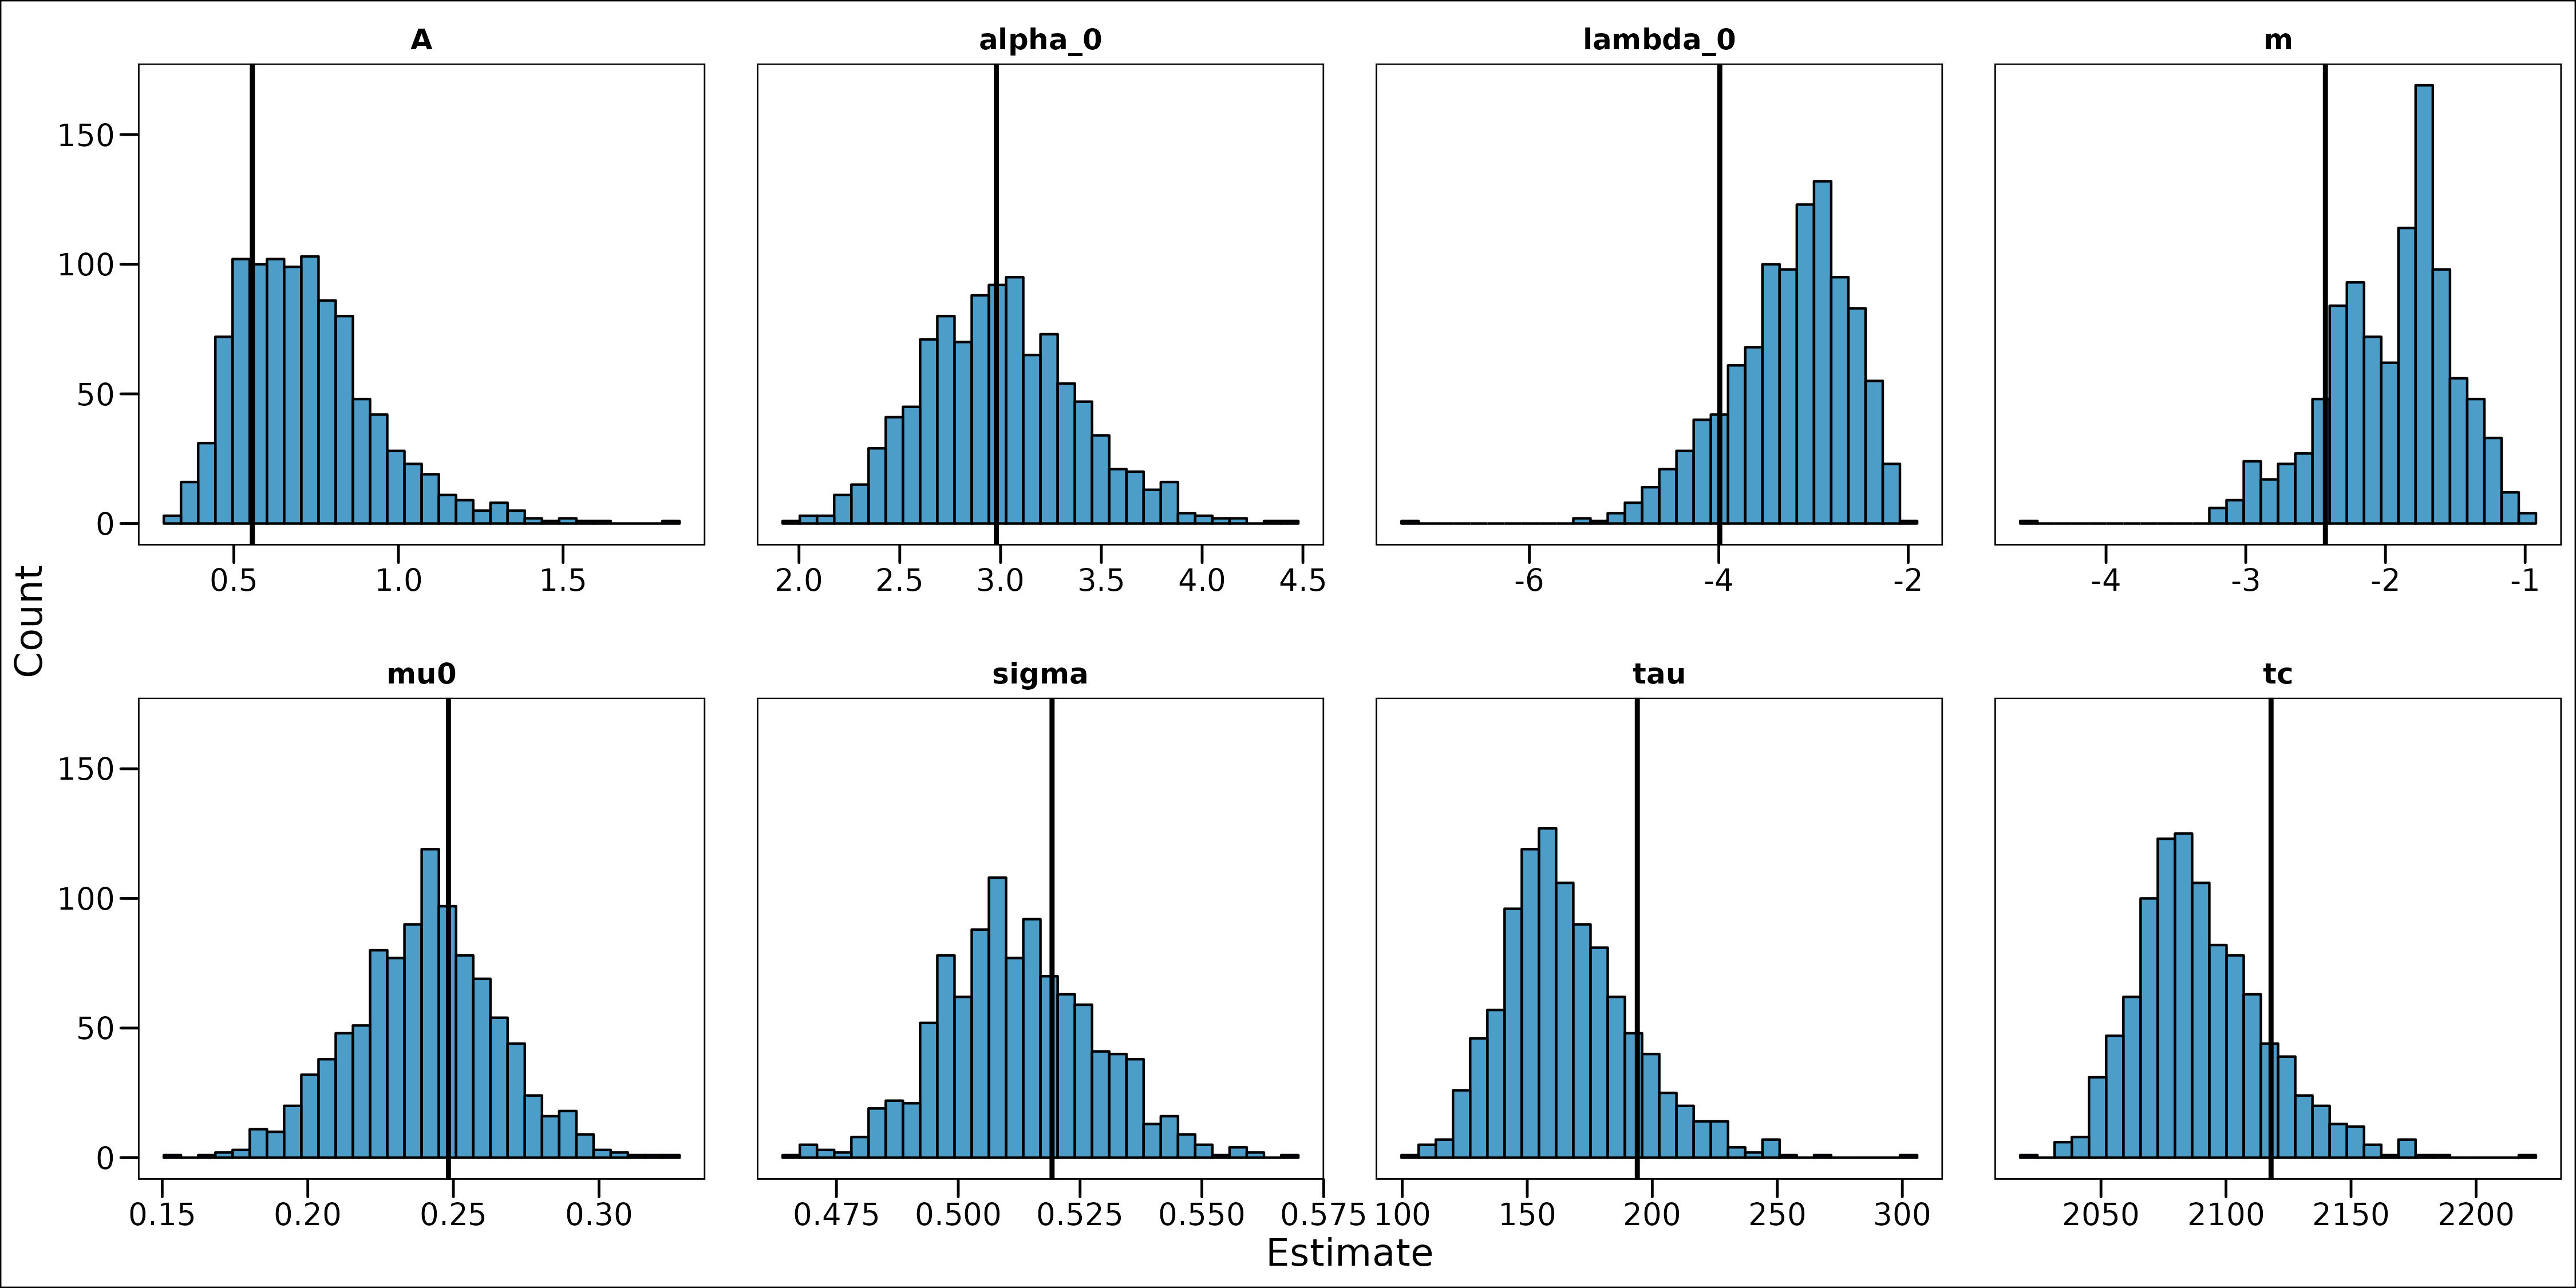
\includegraphics[scale = .095]{figures/estim_tibble_plot.jpeg}
    \caption{Normalized histograms of the estimates from the $t$-diffusion based bifurcation tipping model made with parametric bootstrap.}
    \label{figure:AMOC_parametric_bootstrap}
    \end{center}
\end{figure}\\
In the histograms the estimates from the original fit to the AMOC-data has been overlayed with a dashed line for the respective parameters. Note that for a clearer impression of the distribution, we have removed $7$ extreme estimates of the total $2000$. These estimates have been tabularized and can be seen in appendix \ref{section:benchmark} in table \ref{table:extreme_amoc_estimates}. All the empirical distributions of the estimates cover the values that we estimated from the original data well suggesting an overall good fit of the model.
\subsection{Robustness analysis and the additive noise model}
% \subsection{Tipping in global climate variations}
% Climate physicists have extensively studied ice core data from Greenland as the Greenland ice sheet acts as a sediment for the atmosphere. It is widely accepted that the ratio between the isotopes $^{18}\mathrm{O}$ and $^{16}\mathrm{O}$ is an indicator of the temperature at the time of accumulation. Additionally, $\mathrm{Ca}^{2+}$-ions from dust settle in the ice layer by layer. Unlike the ratio they do not diffuse as much; this allows us to have a finer temporal resolution. We can use calcium-ions instead of the ratio, because there is a negative correlation betwen the logarithm of the log-concetration of the $\mathrm{Ca}^{2+}$-ions and the isotope-ratio. This means that higher calcium-ion concentrations indicate colder global conditions. The ice-core data consists of observations of the oxygen isotope ratio and $\mathrm{Ca}^{2+}$-ion concentrations from $107620$ years before present to $10260$ years before present with a constant temporal resolution of $20$ years. We rescale to kilo years and focus on the observation of the calcium-ion between $86$ kilo years before present (kyrs bp) and $55$ kyrs bp; of course still with $\Delta t = 0.02$. Now, transforming ion-concentrations by $-\log (x)$ is a common practice in chemistry, whence we also consider $-\log([\mathrm{Ca}^{2+}]) - C$, where $C$ is a constant that makes the process have mean zero. We depict the ion-concetration over time. 
% \begin{figure}[h!]
%     \begin{center}
%     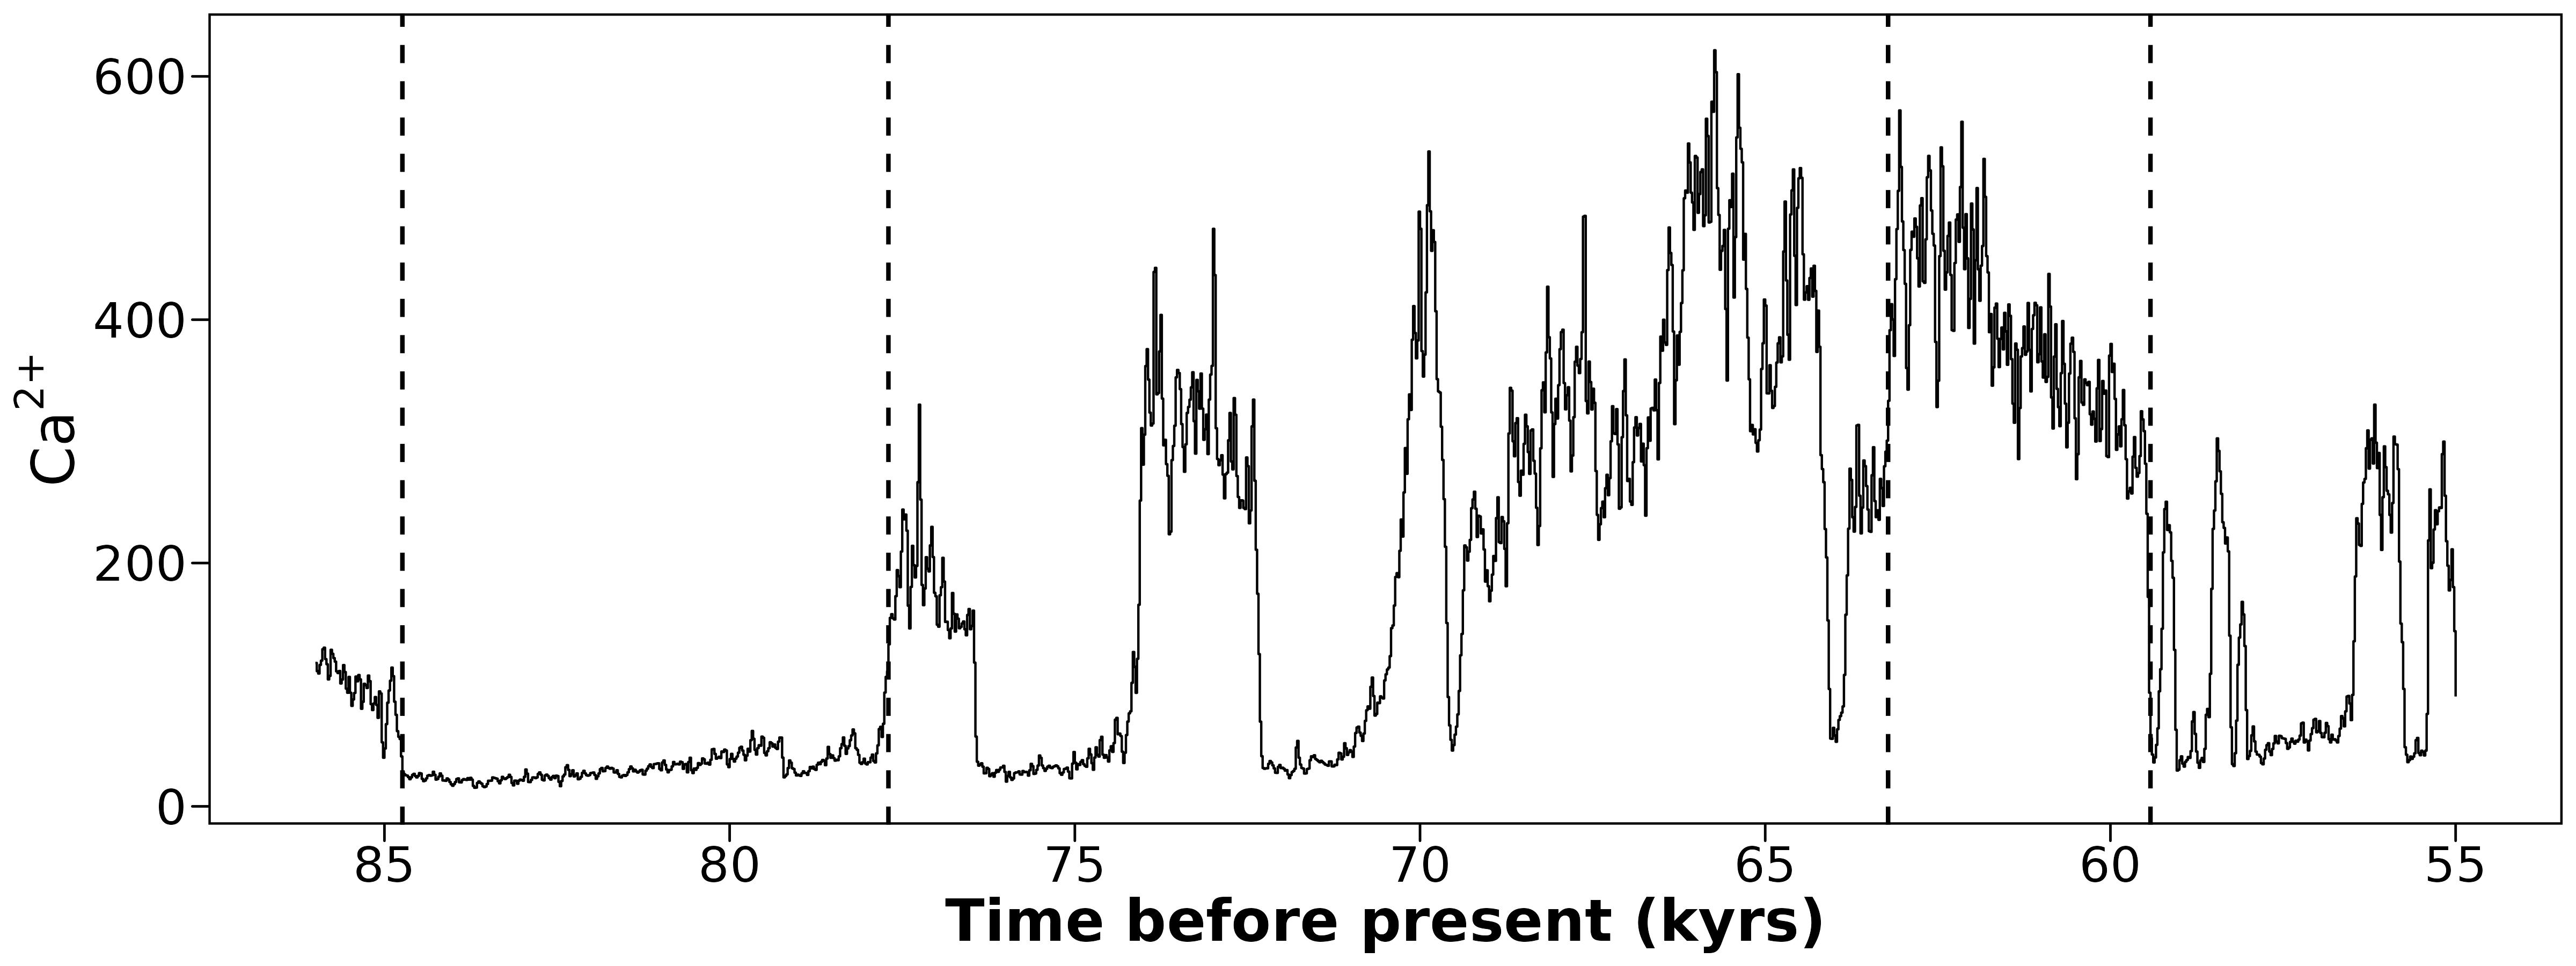
\includegraphics[scale = .075]{figures/ice_core_plot.jpeg}
%     \caption{$\mathrm{Ca}^{2+}$-concetration in the ice sheet in the periode 86 kyrs bp to 55 kyrs bp}
%     \label{figure:Ca_icesheet}
%     \end{center}
% \end{figure}\\
% Looking at graph there are some periods of time where the concetration seem to be in somewhat of a stationary state. We have marked two periods that highlights to such periods by four vertical lines. The two periods we consider concentrations for are $[77.7, 84.74]$ and $[59.42, 63.22]$; these consist of 353 and 191 observations respectively. At the end of the two periods there seem to be a tipping to another state; to make this clear we zoom in on the time periods - note that we add some of the observations after tipping for illustrative purposes
% \begin{figure}[h!]
%     \begin{center}
%     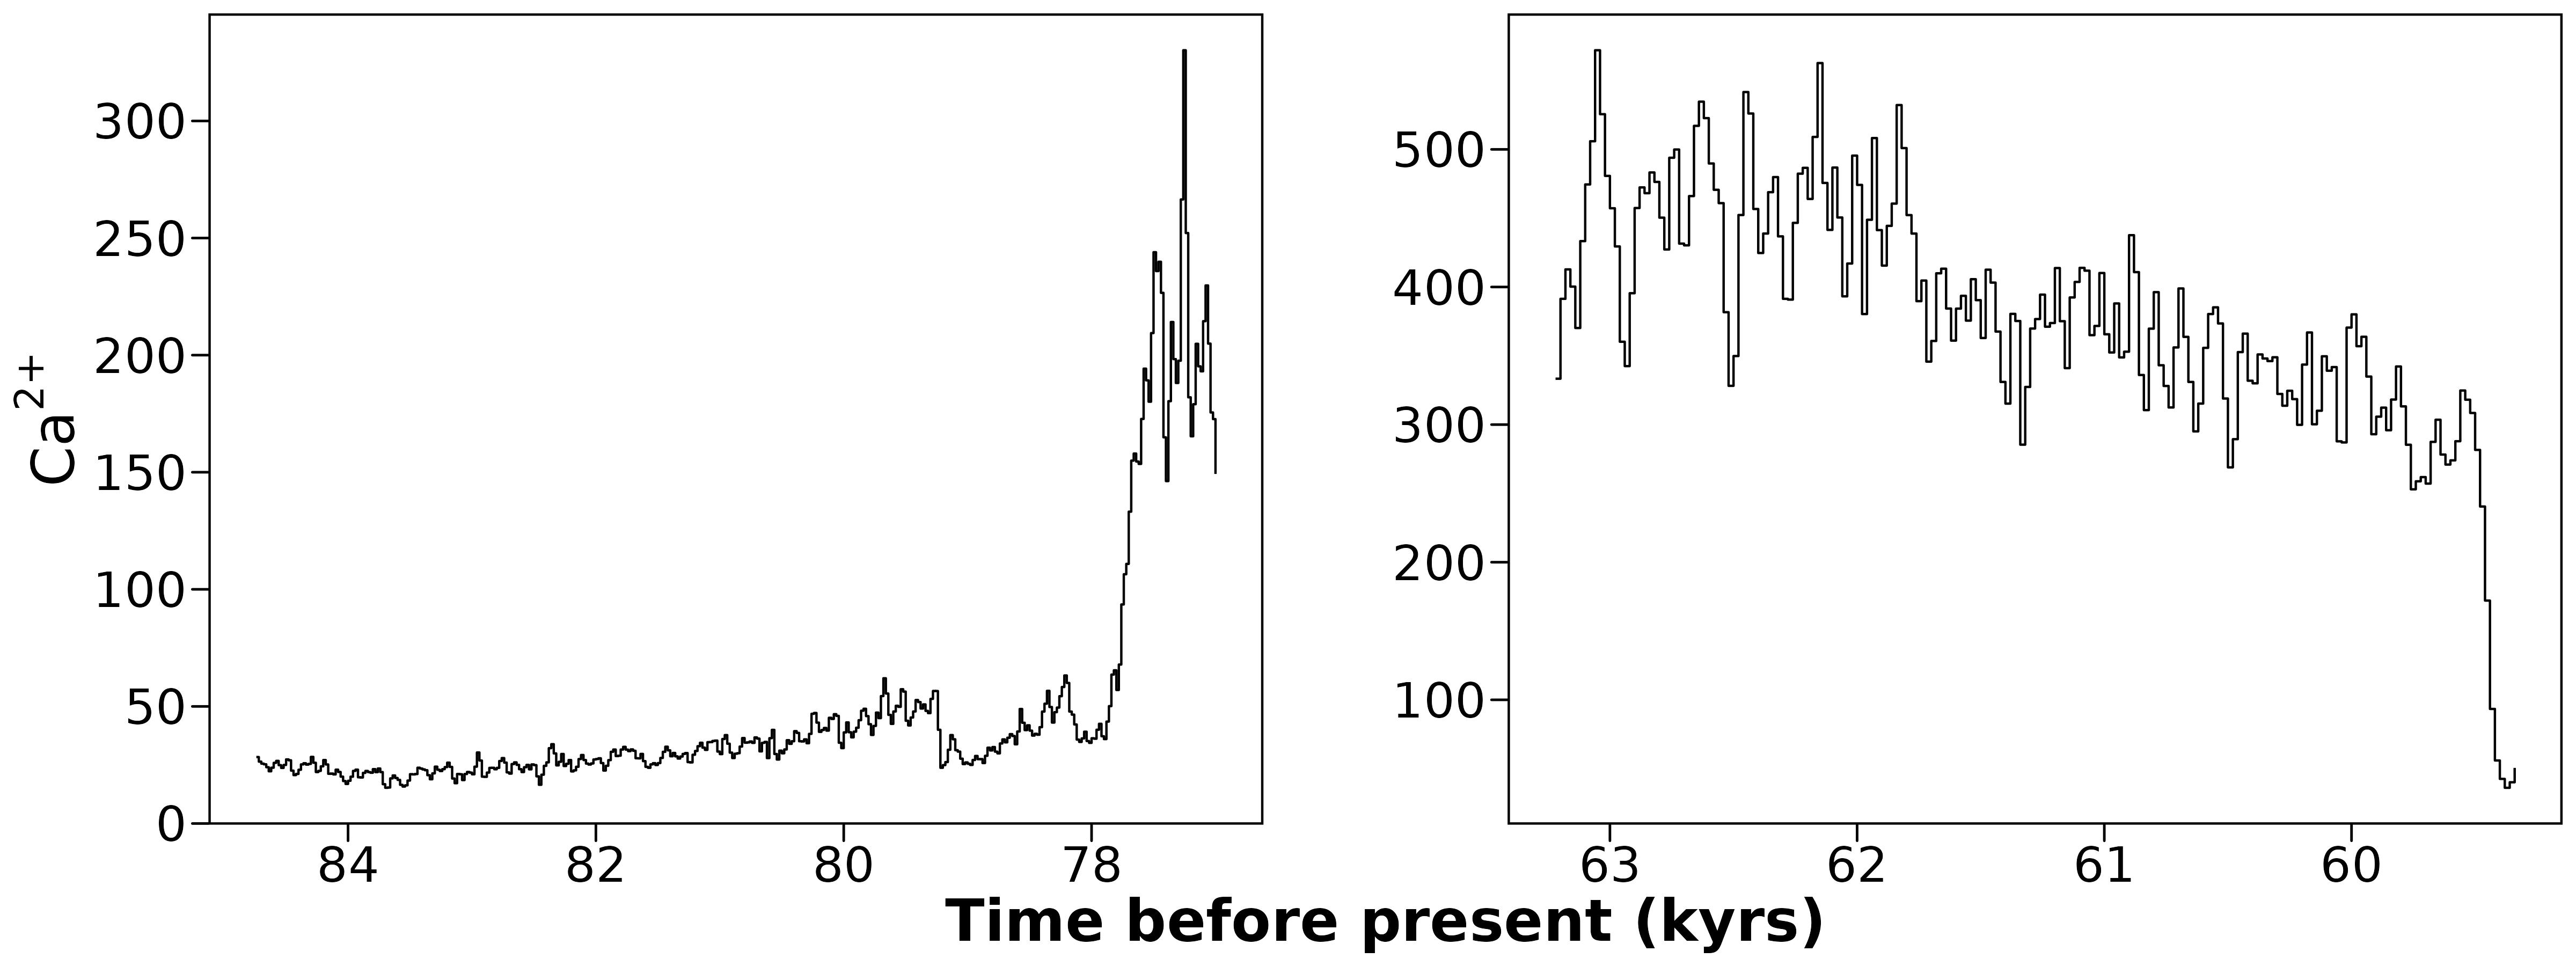
\includegraphics[scale = .075]{figures/ice_core_zoom_plot.jpeg}
%     \caption{Zoom in on the $\mathrm{Ca}^{2+}$-concetration in the ice sheet in the two intervals of interest}
%     \label{figure:Ca_icesheet}
%     \end{center}
% \end{figure}\\
% We analyze both these periods using the mean-reverting geometric brownian motion based model.